%-- Add sections and your outline will be created automatically --%
\section{Restratification after open-ocean deep convection}

\begin{frame}
    \frametitle{Restratification - Setup}
\begin{itemize}
    \item This example is an idealised model of the restratification phase of open-ocean deep convection (OODC).
    \item The setup is taken from Rousset et al. [2009].
    \item Cylinder, radius 250km, height 1km.
\end{itemize}
\begin{figure}
\centering
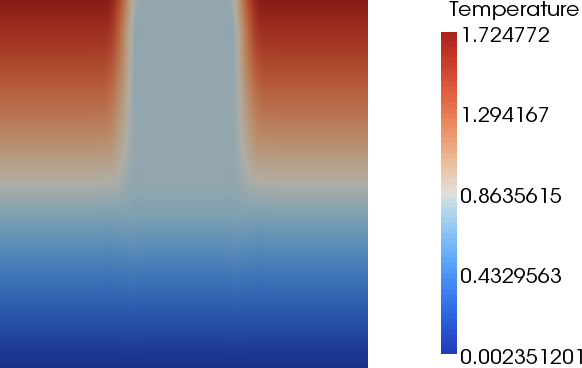
\includegraphics[width=0.4\textwidth]{./restratification_after_oodc/rousset-init.png}
\caption{Cross section of initial temperature distribution.}
\end{figure}
\end{frame}

\begin{frame}
    \frametitle{Restratification - Output}
\begin{figure}
\begin{center}
\subfigure [10 days]{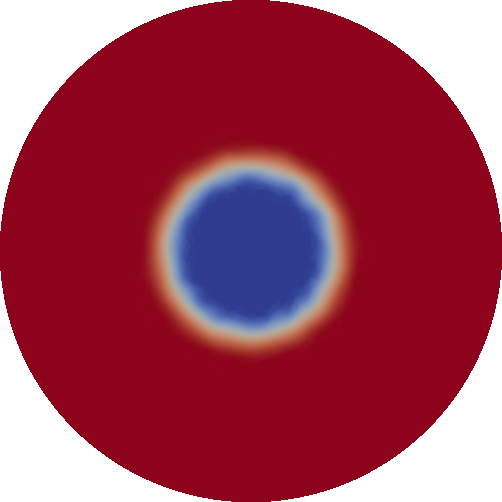
\includegraphics[width=0.2\textwidth]{./restratification_after_oodc/rousset-res5000-depth-40m0003.png}}
\hspace{1cm}
\subfigure [20 days]{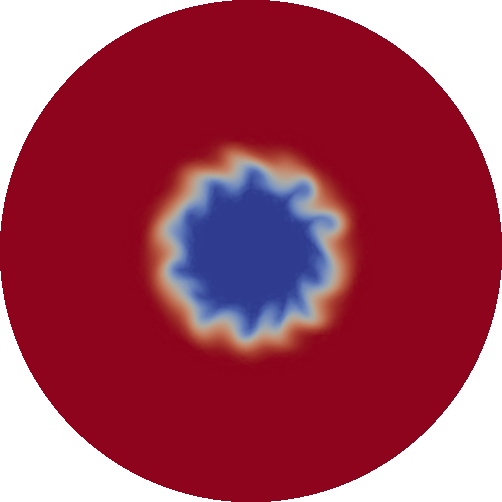
\includegraphics[width=0.2\textwidth]{./restratification_after_oodc/rousset-res5000-depth-40m0005.png}}

\subfigure [30 days]{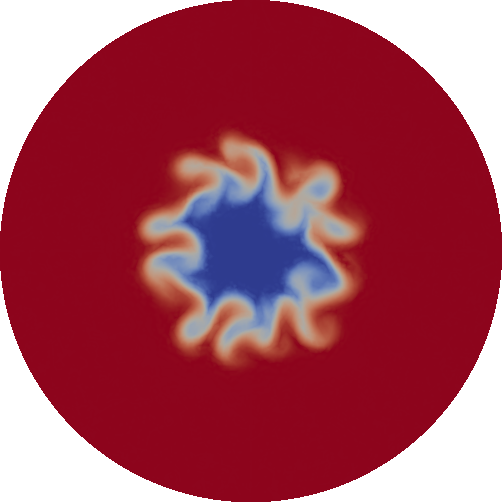
\includegraphics[width=0.2\textwidth]{./restratification_after_oodc/rousset-res5000-depth-40m0007.png}}
\hspace{1cm}
\subfigure [40 days]{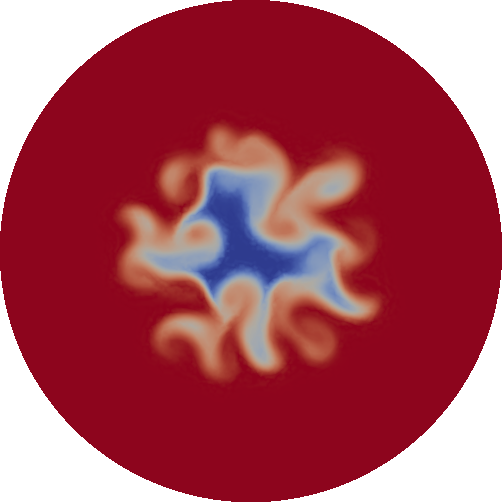
\includegraphics[width=0.2\textwidth]{./restratification_after_oodc/rousset-res5000-depth-40m0009.png}}
\caption{The temperature cross-section at a depth of 40m.}
\label{fig:rousset-40m}
\end{center}
\end{figure}\end{frame}

\begin{frame}
  \frametitle{Restratification - Exercises}
\begin{itemize}
\item How does mesh adaptivity influence the solution?
\item Fixed mesh resolution size - what happens as you increase/decrease the resolution?
\item Discretisation of temperature - what changes between DG, CG and CV?
\item Scaling - how far can you push the parallisation of this run, with and without adaptivity?
\end{itemize}
\end{frame}






